\section{Key Ideas}
\begin{lucido}[Research Problem]
	\begin{enumerate}
		\setbeamertemplate{enumerate items}[square]
		\item  An operator allowing to generalize the current ``grouping'' and ``nesting'' is missing. Nevertheless, current (G)DBMSs allow to express nesting operations, but their query languages' plans do not allow to optimize the whole process by combining the following tasks:
		\begin{itemize}
			\item \alert{path joins} separately for both patterns.
			\item \alert{grouping} to create an id collection over the matched elements.
		\end{itemize}
		\item The general nesting algorithm could lead to an exponential evaluation time.
	\end{enumerate}
\end{lucido}

\begin{lucido}[Use Case]
	\begin{columns}[onlytextwidth]
		\begin{column}{.45\textwidth}
			\begin{figure}
				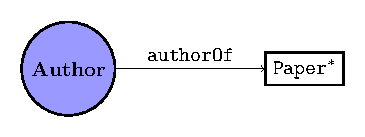
\includegraphics[scale=0.6]{../images/nesting/patterns/00_vertex_pattern.pdf}
				\begin{center}
					Vertex Pattern
				\end{center}
			\end{figure}
		\end{column}
		\hfill
		\begin{column}{.45\textwidth}
			\begin{figure}
				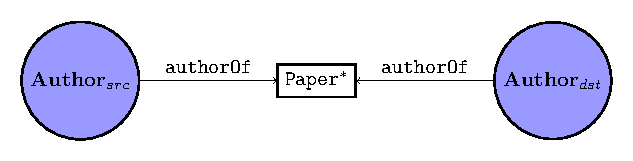
\includegraphics[scale=0.45]{../images/nesting/patterns/00_path_pattern.pdf}
				\begin{center}
					Edge Pattern
				\end{center}
			\end{figure}			
		\end{column}
	\end{columns}
	\begin{center}
		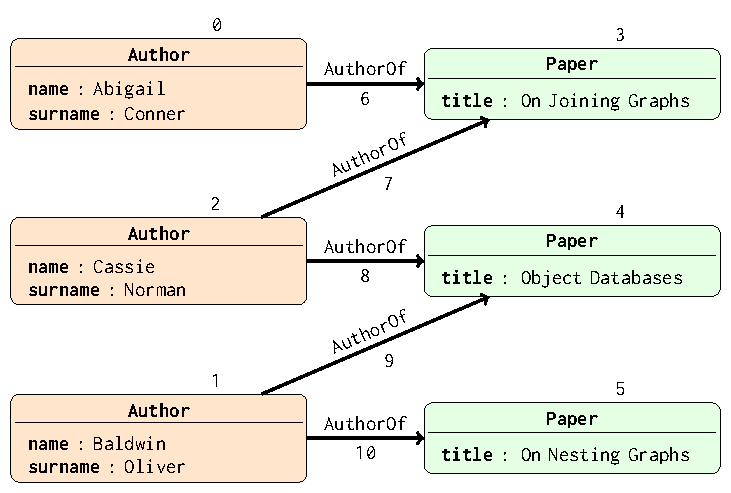
\includegraphics[height=.5\textheight]{../images/nesting/patterns/04bibliography.pdf}\\
		Input Bibliography Network
	\end{center}
\note{In questo problema specifico, imponiamo che 1) esista un sottografo in comune alle due componenti, e 2) che ogni sorgente e destinazione dell'arco possa corrispondere ad un vertice che \`e stato precedentemente annidato.}
\end{lucido}

